All Monte-Carlo-based predictions rely on the best estimate for a set
of parameters $\hat{\vect{\theta}}$. These parameters can be
theoretical in nature, such as the cross section to which the
prediction is scaled, or intrinsic to the ATLAS detector, such as the
efficiency for selecting an electron. The uncertainties on these
parameters are propagated to uncertainties on event yields in the
signal and control regions, and as we will see in the following
chapter, these uncertainties are ultimately propagated to an error on
the measured VBF signal strength. Uncertainties are always computed at a
working point corresponding to $\pm 1\sigma$ and propagated to the
statistical fit as such.

\subsection{Theoretical sources}

Monte Carlo generators are approximate models for any scattering
process. To assess theoretical uncertainties, approximations are
varied, and the resulting change in the prediction is
quantified. The following sources of uncertainty are considered:
parton distribution function (PDF), QCD scale, parton showering
program, hard-scattering program, and underlying event tune. Depending
on the source, these uncertainties are split into two kinds:
normalization and acceptance. Normalization uncertainties are those
that vary the overall normalization of a prediction without changing
the underlying distributions. Acceptance uncertainties are computed
for sources that change kinematic distributions and therefore
selection efficiences. Because the BDT spectrum spans a large and
relatively unknown region of phase space, acceptance uncertainties are
computed separately in each BDT fit bin.

Varying the factorization ($\mu_F$) and renormalization scales
($\mu_R$) probes sensitivity to the corrections from the next order in
the perturbative expansion. For the VBF process, $\mu_F$ and $\mu_R$
are varied up and down by a factor of two, and the resulting change in
event rates in the signal region is on the order of 0.5\%. Since the
scale change impacts the BDT input distributions associated with tag
jets, namely \mjj and \dyjj, there is a distortion of the BDT
spectrum of [1\%,3\%,3\%] in BDT bins. 

The PDF uncertainty is also evaluated for the VBF signal process. 
Comparing the baseline PDF \ctten to \nnpdf (reference), the
difference in event yields in the BDT SR is found to be 4\%, with a
negligible dependence on the BDT score. The baseline hard-scattering
generator is \POWHEG which simulates the VBF process at NLO in
QCD. Another generator, \aMCATNLO, utilizes a different prescription
for matching the HS and the PS, and in order to ascertain the
uncertainty associated with the default prescription, the predictions
of the two generators are compared. Although the shape variation of
the BDT distribution is negligible, \aMCATNLO predicts 4\% more events
than \POWHEG in the BDT SR, which is assigned as a normalization
uncertainty. Additionally, uncertainties associated with corrections
from higher order EW corrections are assessed by turning these
corrections on and off in the generator \VBFNLO. These corrections are
observed to have little impact on the shape of the BDT spectrum, and
increase the overall cross section by 3.5\%, a correction which is
already accounted for in the NLO cross section calculation to which
the baseline prediction is scaled~\ref{chap:analysis:sec:data_mc}.

The dominant uncertainty on signal is associated with the parton
shower program. Comparing the baseline program, \PYTHIA, to \HERWIG,
the difference in the event yield in the signal region is 3.4\%. The
distortion of the BDT spectrum is large due to the fact that the BDT
input \pttot is highly sensitive to the soft
jet activity in an event. Though the effect is as large as 50\% in
the \pttot distribution, in the BDT distribution the largest
difference is 10\% in the highest BDT bin, because the BDT selects the
region of phase space associated with the core of the \pttot
distribution. 

As discussed in
section~\ref{chap:analysis:sec:dd_backgrounds:subsec:top}, the
theoretical uncertainties
for \ttbar~and ST are computed by varying the PDF, QCD scale, parton
shower, and the hard-scattering generator. Because this background is
normalized with a control region, the change in the extrapolation
factor $\alpha = \frac{N_{top,MC}^{SR}}{N_{top,MC}^{CR}}$
(equation~\ref{chap:analysis:equation:top_est}) is measured in order to
assess the uncertainty on the signal region event rate. The dominant
uncertainty source has been found to be the hard-scattering generator,
derived from a comparison of \MCATNLO and \ALPGEN. In the respective
BDT fit bins, these uncertainties are 10\%, 12\%, and 21\%.

Non-resonant \wwtwoj production is a large background,
contributing \textapprox{19\%} of the total background in the \emme SR and \textapprox{9\%} in
the \eemm SR. QCD \wwtwoj rates are predicted with an
inclusive \SHERPA sample normalized to the NLO \MCFM cross section. To
assess the hard-scattering and QCD scale uncertainties, \MADGRAPH interfaced
with \PYTHIA 6 for showering is used. The sample which is generated is
also inclusive, with up to three partons generated at the matrix
element
level. These final state partons are then showered in \PYTHIA with the
MLM matching scheme (reference) at a scale of 20~\gev. The PDF in
both \MADGRAPH and \PYTHIA is \cteqsixl, and the underlying event tune
is AUET2B (reference). 

The hard-scattering uncertainty is computed by comparing
the truth level predictions of \MADGRAPH to those of the \SHERPA. In
an approach similar to the one used in the evaluation of top theory
uncertainties, the BDT inputs are
evaluated at truth level, and the resulting distortion of the BDT
spectrum is taken as an uncertainty. For the comparison, the two truth level
samples are scaled to the integrated luminosity with their respective
cross sections. The inclusive \MADGRAPH cross section computed after showering
is 4.55~pb, which is significantly smaller than the cross section to
which the \SHERPA prediction is scaled: 5.679~pb. However, because the
fraction of events with two or more jets is larger in \MADGRAPH, the
uncertainty after requiring two jets is mitigated. Displayed in
figure~\ref{chap:analysis:fig:qcdww_gen_uncert} is the truth level BDT
response. In light of the differences, uncertainties of 14\%, 8\%, and
12\% are assigned.

\begin{figure}[h]
    \centering
    \subfigure[QCD \ww]{
    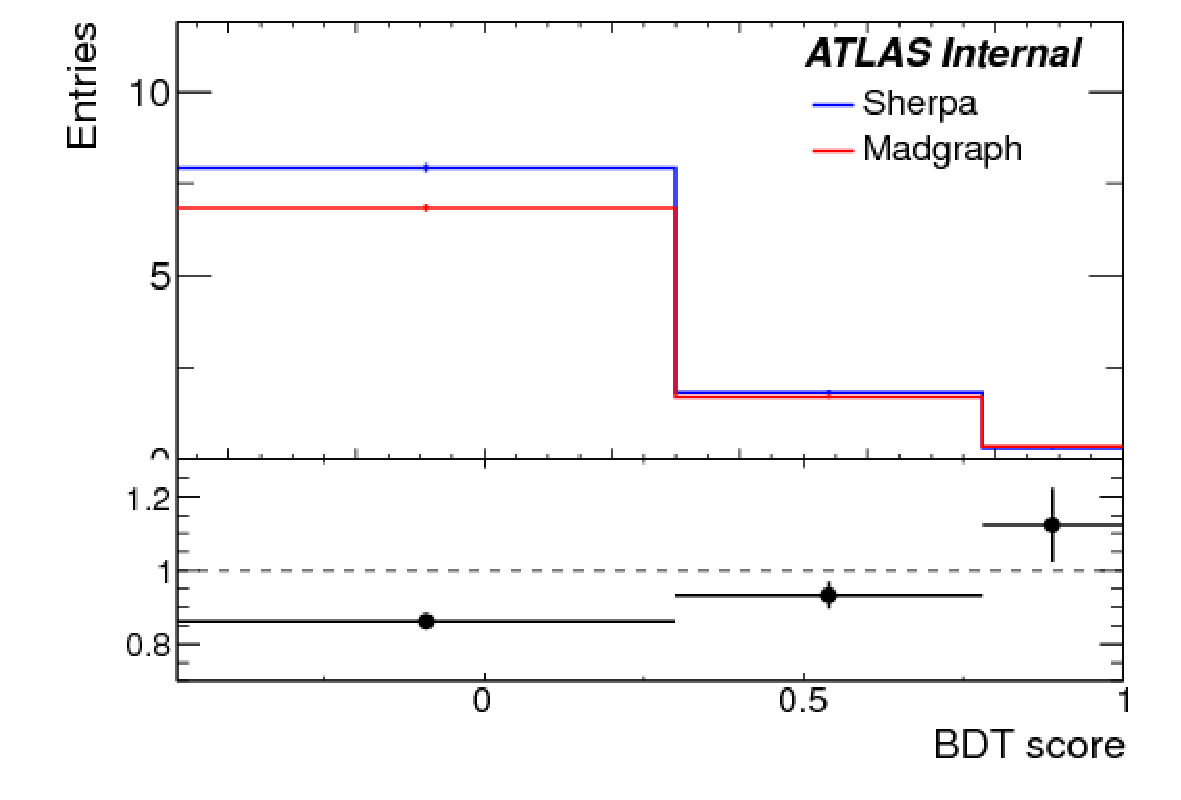
\includegraphics[width=0.45\textwidth]{analysis/ww/ww_shape_sys_qcd.pdf}
    \label{chap:analysis:fig:qcdww_gen_uncert}
    }
    \subfigure[EW \ww]{
    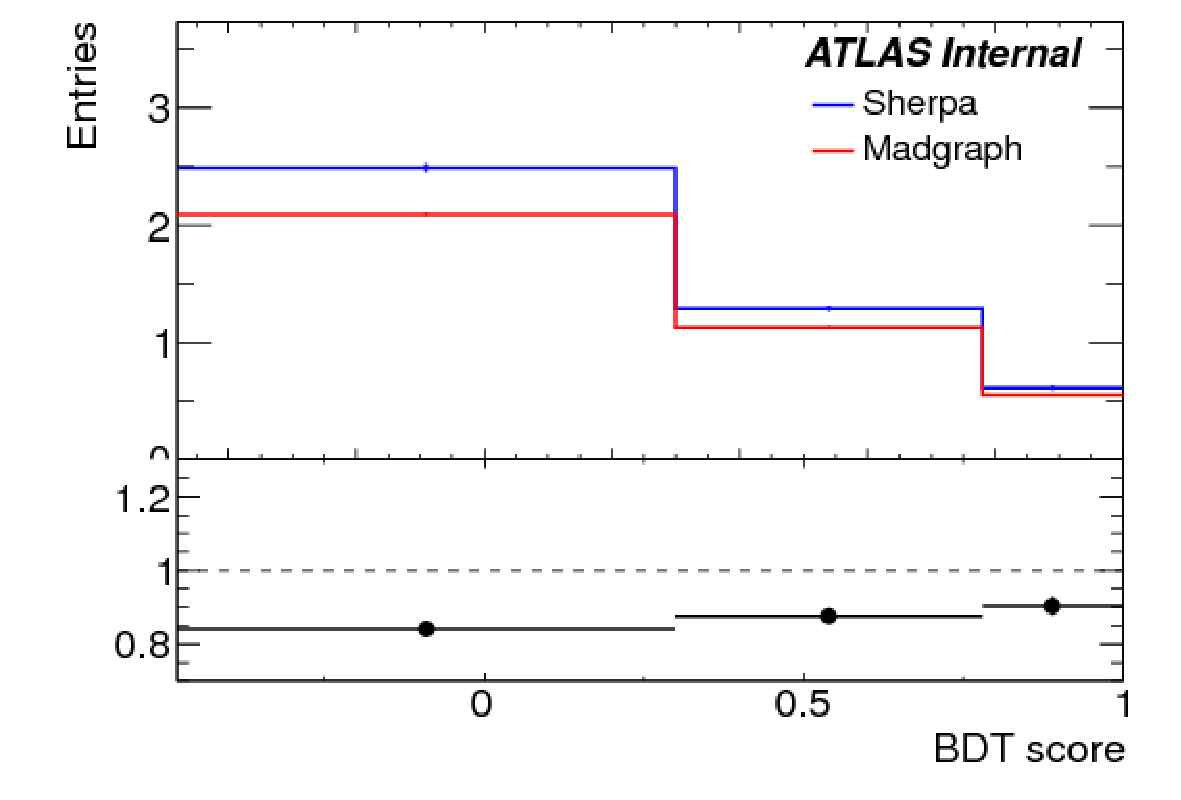
\includegraphics[width=0.45\textwidth]{analysis/ww/ww_shape_sys_ew.pdf}
    \label{chap:analysis:fig:ewww_gen_uncert}
    }
    \caption[Comparison of \MADGRAPH and \SHERPA predictions
    for \ww.]{Comparison of \MADGRAPH and \SHERPA predictions in the
    \emme BDT signal region for~\subref{chap:analysis:fig:qcdww_gen_uncert}
    QCD \ww and~\subref{chap:analysis:fig:ewww_gen_uncert} EW \ww
    processes. Comparison is at truth-level, and the difference
    between the two generators is assigned as a modelling uncertainty.}
\label{chap:analysis:fig:ww_gen_uncert}
\end{figure}

To assess the uncertainty from the choice of QCD scale, the
factorization and renormalization scales in \MADGRAPH,
which are varied dynamically event-by-event, are coherently scaled up
and down by a factor of two. The resulting samples are scaled to their
respective post-parton-showering cross sections, and the signal region
differences are computed. With the scale set to 
$\mu_R=\mu_F=\mu_{\textrm{default}}/2$, the
predicted number of events in the SR is $27\%$ higher than the default
scale choice, while with $\mu_R=\mu_F=2\mu_{\textrm{default}}$, the
prediction
falls by $2.6\%$. The larger of the two, $27\%$, is assigned as the
uncertainty, which is consistent with the LO $\sigma(WW)$
uncertainty computed at \sqrts$=7$~\tev ~\cite{bib:Melia:2011dw}, though in a
looser phase space region. Because the QCD scale variations induce
small shape differences in the BDT input distributions, the
uncertainty is flat across the BDT fit bins. Additional QCD \ww uncertainties are
summarized in table~\ref{chap:analysis:tab:ww_theory_uncerts}.

\begin{table}
\begin{center}
\renewcommand{\arraystretch}{1.2}
%\resizebox{0.8\textwidth}{!}{
    \begin{tabular}{ l | c | c }
    \hline
    Source & QCD \ww & EW \ww \\
    \hline \hline
    Generator modeling & (12\%,8\%,12\%) & (16\%,12\%,10\%) \\
    QCD scale & 27\% & 10\% \\
    PDF ($\sigma$) & 4\% & 3\% \\
    PDF (acceptance) & 2\% & $-$ \\
    QCD-EW interference & $-$ & 2\% \\
    Higgs interference & $-$ & 1.2\% \\
    \hline
    \end{tabular}
%}
\caption[Summary of \ww theory uncertainties.]{Summary of the
    theoretical uncertainties assigned to the QCD and EW \ww
    background processes.}
\label{chap:analysis:tab:ww_theory_uncerts}
\end{center}
\end{table}

For EW \ww, a hard-scattering modeling uncertainty is computed by comparing
the prediction of \SHERPA to that of an exclusive two jet \MADGRAPH
sample interfaced
with \PYTHIA. The cross section computed in \MADGRAPH is 27.37~fb,
30\% lower than that of \SHERPA, resulting in fewer events
predicted. A comparison of the absolute predictions for the two
generators is shown in
figure~\ref{chap:analysis:fig:ewww_gen_uncert}, corresponding to
uncertainties of 16\%, 12\%, and 10\% in BDT bins.

The QCD scale uncertainty is computed at LO
in~\cite{bib:Jager:2006zc}. The uncertainty is computed in a generic
VBF phase space region with cuts on \dyjj and \mjj. Such a region is
expected to significantly overlap with the SR defined by the BDT. The
resulting uncertainty, computed by varying $\mu_F$ and extracting the
cross section, is 10\%.

Remaining theory uncertainties for EW \ww are shown in
table~\ref{chap:analysis:tab:ww_theory_uncerts}. The uncertainty from
interference
between EW \ww and Higgs-mediated \ww is computed by comparing the
cross section of \ww and \hww diagrams without interference to the
corresponding cross section with interference. At a Higgs mass
hypothesis of $m_H = 125$~\gev, the uncertainty is 1.2\%, while at
$m_H = 150$~\gev, the uncertainty is 6.4\%. Because these are small
with respect to the modeling and QCD scale uncertainties, they are
neglected in the fit. An uncertainty due to interference between QCD
and EW \ww processes is evaluated in a similar way and found to
be \textapprox{2\%}. This, too, is neglected in the fit.

Gluon-gluon-fusion Higgs production (ggF) is a large background in the
most sensitive BDT bins. In order to estimate the uncertainties from
higher order terms in the perturbative expansion, the $\mu_F$ and
$\mu_R$ are independently varied in \MCFM. Since the final statistical
result is derived from a likelihood across the jet bins, it is
important to correctly correlate the normalization uncertainty for
each jet bin. Moreover, applying a central jet veto effectively limits
the phase space to the exclusive two jet bin, calling for the
uncertainty to be computed for such a region. An approach that
accounts for these considerations has been proposed by Stewart and
Tackmann~\cite{bib:Stewart:2011cf}. The exclusive cross section can be
expressed as 

\begin{equation}
\sigma_{\textrm{2j}} = \sigma_{\geq\textrm{2j}} - \sigma_{\geq\textrm{3j}}
\end{equation}

where $\sigma_{\geq\textrm{2j}}$ ($\sigma_{\geq\textrm{3j}}$) is the
inclusive two (three) jet cross section. To a good approximation,
$\sigma_{\geq\textrm{2j}}$ and $\sigma_{\geq\textrm{3j}}$ can be
considered to be uncorrelated, and therefore the uncertainty on the
exclusive two jet cross section can be computed as the quadrature sum
of the two inclusive uncertainties. To ascertain the uncertainties
in \MCFM, the scales are varied, and the BDT preselection is
applied. For the inclusive 2j bin, the CJV is not applied, and for the
inclusive 3j bin, the CJV is inverted. The resulting relative
uncertainties are $\Delta_{\geq\textrm{2j}} = 22\%$ and
$\Delta_{\geq\textrm{3j}} = 118\%$, corresponding to a normalization
uncertainty of $\Delta_{\textrm{2j}} = 34\%$ in the BDT signal
region. In addition, the shape variation with QCD scale is computed
and found to be [+2.4/-2.5,+2.6/-2.5,+13/-12]\% in the BDT fit
bins. 

Uncertainties on ggF from other sources are small with respect to the
QCD scale uncertainty. The PDF uncertainty is 8\%. The underlying
event and parton shower uncertainty, computed by comparing \HERWIG
showering to the baseline program \POWHEG, is a flat 15\% across the
BDT bins. 

For \ZDYll processes, because a data-driven approach is used, the only
prediction from MC simulation is the relative rate in the last two BDT
bins. Three sources of uncertainty
on this quantity have been considered: (1) QCD scale, (2) parton
shower, (3) PDF. Of these three sources, evaluated with \SHERPA, the
largest is QCD scale, corresponding to an uncertainty of 11\% in the
last BDT bin. The other two sources are neglected. In the \emme
channel, the \Ztautaunody normalization is constrained from a control
region, which, due to limited statistics in this region, results in a
large statistical uncertainty of 30\%. Due to the negligible
contribution of this background in the most sensitive BDT bins and to
the fact that the theory uncertainties are {\it a priori} assumed to
be smaller than the statistical uncertainties, theory uncertainties
are not computed for this background component. 

The theory uncertainties for the remaining backgrounds, which are
small in the SRs, will not be discussed here, as they have little
impact on the statistical result. 

\subsection{Instrumental sources}

Systematic uncertainty sources due to the reconstruction and identification of
electrons, muons, jets, and missing transverse energy are also
considered. These sources are evaluated by varying the relevant
parameter in simulation and then measuring the resulting change in the
event yields in the BDT signal region. Because the uncertainties are
generally binned in the \pt~and $\eta$ of the object, the event yield
variations are evaluated separately in each BDT bin and correlated.

As discussed in section~\ref{chap:analysis:sec:objects}, the
efficiencies associated with lepton selection are corrected with
data. The uncertainties on these scale factors, summarized in
table~\ref{chap:analysis:tab:lepton_eff}, are split into two
uncorrelated components associated with the isolation SF and
the identification SF. Propagated to the event yields in the SR, these
two uncertainties are both less than 1\% for signal and background
(tables~\ref{chap:analysis:tab:exp_sys_df}
and~\ref{chap:analysis:tab:exp_sys_sf}). The remaining lepton
uncertainties are due to the momentum scale and resolution calibrations,
discussed in chapter~\ref{chap:reco}. For both signal and background event
yields, these uncertainties are $\leq 0.5\%$ for electrons and
negligible for muons. 

\begin{table}[h!]
\begin{center}
\renewcommand{\arraystretch}{1.2}
\resizebox{1.0\textwidth}{!}{
\begin{tabular}{l || c c | c c c c c c }
\hline
Uncertainty & \multirow{2}{*}{Signal} & Total &
\multirow{2}{*}{top} & \multirow{2}{*}{$WW$} & \multirow{2}{*}{ggF} &
Non-$WW$ & \multirow{2}{*}{\ZDY} & \multirow{2}{*}{Fakes} \\
Source & & Back & & & & Diboson & & \\
\hline
$\textrm{Trigger}$ & 0.5 & 0.5 & 0.5 & 0.5 & 0.5 & 0.8 & 0.6 & - \\
$\textrm{electron SF}$ & 0.8 & 0.8 & 0.8 & 0.9 & 0.9 & 1.1 & 1.1 & -
\\
$\textrm{electron reso.}$ & 0.1 & 0.5 & 0.2 & - & - & 1.5 & 4.7 & - \\
$\textrm{electron scale}$ & 0.2 & 0.5 & 0.6 & 0.5 & 0.3 & 1.6 & 2.7 &
- \\
$\textrm{electron iso.}$ & 0.7 & 0.6 & 0.7 & 0.7 & 0.8 & 0.8 & 0.8 & -
\\
$\textrm{muon SF}$ & 0.3 & 0.3 & 0.3 & 0.3 & 0.3 & 0.3 & 0.3 & - \\
$\textrm{muon reso.}$ & 0.1 & - & 0.2 & 0.1 & 0.1 & 0.1 & 0.4 & - \\
$\textrm{muon scale}$ & - & 0.1 & 0.1 & 0.2 & - & - & 0.4 & - \\
$\textrm{muon iso.}$ & 0.8 & 0.7 & 0.8 & 0.8 & 0.8 & 0.9 & 0.9 & - \\
$\textrm{JES flavor}$ & 0.8 & 0.9 & 0.7 & 2.8 & 3.0 & 3.5 & 0.3 & - \\
$\textrm{JES}~\eta~\textrm{model}$ & 2.8 & 4.7 & 3.9 & 10.2 & 5.9 &
1.3 & 6.6 & - \\
$\textrm{JES}~\eta~\textrm{stat.}$ & 0.4 & 0.8 & 0.9 & 1.3 & 0.8 & 1.8
& 0.2 & - \\
$\textrm{JES flav. response}$ & 0.7 & 0.3 & 0.2 & 2.1 & 1.9 & 2.9 &
4.7 & - \\
$\textrm{JES detector}$ & 0.3 & 0.7 & 1.1 & 0.9 & 0.7 & 0.9 & - & - \\
$\textrm{JES pileup}~\pt$ & - & 0.6 & 0.2 & 0.6 & 0.3 & 0.1 & 4.3 & -
\\
$\textrm{JES high}~\pt$ & - & 0.5 & - & - & - & - & 3.8 & - \\
$\textrm{JES pileup}~\rho$ & 0.4 & - & 0.5 & 1.5 & 1.4 & 0.6 & 5.6 & -
\\
$\textrm{JES modelling}$ & 1.1 & 1.7 & 1.9 & 3.9 & 3.4 & 5.4 & 2.6 & -
\\
$\textrm{JES}~\left \langle \mu \right \rangle$ & - & 0.5 & 0.3 & 0.4
& 0.6 & 2.5 & 0.5 & - \\
$\textrm{JES}~\nvtx$ & 0.1 & 0.3 & 0.2 & 0.7 & 0.7 & 2.8 & 3.2 & - \\
$\textrm{JES AFII}$ & - & - & - & - & - & - & - & - \\
$b\textrm{-tag SF}$ & - & 2.4 & 6.5 & 0.1 & - & - & - & - \\
$\textrm{light tag SF}$ & 1.3 & 1.3 & 1.2 & 1.7 & 1.9 & 1.8 & 1.6 & -
\\
$c\textrm{-tag SF}$ & 0.4 & 0.2 & 0.2 & 0.3 & 0.2 & 0.3 & 0.2 & - \\
$\calomet~\textrm{scale}$ & - & 0.3 & - & - & - & - & 2.2 & - \\
$\calomet~\textrm{reso.}$ & - & - & - & - & - & - & - & - \\
$\trkmet~\textrm{scale}$ & 0.3 & 2.2 & 2.6 & 2.0 & 1.0 & 0.3 & 6.6 & -
\\
$\trkmet~\textrm{reso.}$ & 0.6 & 3.6 & 4.1 & 1.4 & 2.2 & 15.7 & 9.0 &
- \\
$\textrm{di-jet fake rate}$ & - & 1.9 & - & - & - & - & - & 14.5 \\
$\textrm{fake rate}~\mu$ & - & 1.6 & - & - & - & - & - & 12.0 \\
$\textrm{fake rate}~e$ & - & 2.2 & - & - & - & - & - & 17.1 \\
$\left \langle \mu \right \rangle~\textrm{re-scale}$ & 1.2 & 0.5 & 0.8
& 0.4 & 0.9 & 3.6 & 4.4 & - \\
\hline
\end{tabular}
}
\caption[Instrumental uncertainty summary in the \emme
  channel.]{Instrumental uncertainty summary in the \emme channel.}
\label{chap:analysis:tab:exp_sys_df}
\end{center}
\end{table}

\begin{table}[p!]
\begin{center}
\renewcommand{\arraystretch}{1.2}
\resizebox{0.9\textwidth}{!}{
\begin{tabular}{l || c c | c c c c c c }
\hline
Uncertainty & \multirow{2}{*}{Signal} & Total &
\multirow{2}{*}{top} & \multirow{2}{*}{$WW$} & \multirow{2}{*}{ggF} &
Non-$WW$ & \multirow{2}{*}{\ZDY} & \multirow{2}{*}{Fakes} \\
Source & & Back & & & & Diboson & & \\
\hline
$\textrm{Trigger}$ & 1.2 & 0.5 & 1.1 & 1.2 & 1.2 & 0.6 & 0.1 & - \\
$\textrm{electron SF}$ & 0.6 & 0.3 & 0.6 & 0.7 & 0.6 & 1.9 & 0.1 & -
\\
$\textrm{electron reso.}$ & - & 0.4 & 0.5 & 0.1 & 0.3 & 0.3 & 0.5 & -
\\
$\textrm{electron scale}$ & - & 0.1 & 0.1 & 1.0 & - & 3.4 & 0.2 & - \\
$\textrm{electron iso.}$ & 0.6 & 0.3 & 0.5 & 0.6 & 0.6 & 1.4 & 0.1 & -
\\
$\textrm{muon SF}$ & - & - & - & - & - & - & - & - \\
$\textrm{muon reso.}$ & - & 0.1 & - & 0.4 & - & - & 0.1 & - \\
$\textrm{muon scale}$ & - & - & 0.2 & - & - & - & 0.1 & - \\
$\textrm{muon iso.}$ & 1.0 & 0.4 & 1.0 & 1.0 & 1.0 & 0.4 & 0.1 & - \\
$\textrm{JES flavor}$ & 1.9 & 1.1 & 0.6 & 4.4 & 4.0 & 18.0 & 0.1 & -
\\
$\textrm{JES}~\eta~\textrm{model}$ & 5.2 & 3.2 & 5.4 & 9.8 & 8.0 &
10.2 & 1.2 & - \\
$\textrm{JES}~\eta~\textrm{stat.}$ & 0.6 & 0.6 & 0.9 & 1.1 & 0.6 & 4.7
& 0.3 & - \\
$\textrm{JES flav. response}$ & 1.4 & 0.9 & 0.7 & 2.3 & 2.5 & 14.2 &
0.1 & - \\
$\textrm{JES detector}$ & 0.9 & 0.7 & 1.0 & 0.6 & 0.8 & 7.4 & 0.3 & -
\\
$\textrm{JES pileup}~\pt$ & - & 0.4 & - & 0.1 & 0.3 & 0.9 & 0.6 & - \\
$\textrm{JES high}~\pt$ & - & 0.2 & - & - & - & - & 0.3 & - \\
$\textrm{JES pileup}~\rho$ & 0.4 & 0.5 & 0.1 & 2.0 & 1.0 & 10.9 & - &
- \\
$\textrm{JES modelling}$ & 2.1 & 1.6 & 1.4 & 4.6 & 4.2 & 15.2 & 0.6 &
- \\
$\textrm{JES}~\left \langle \mu \right \rangle$ & - & 0.5 & 0.1 & 1.1
& 0.7 & 3.3 & 0.4 & - \\
$\textrm{JES}~\nvtx$ & - & 0.4 & 0.1 & 1.1 & 0.3 & 7.0 & 0.3 & - \\
$\textrm{JES AFII}$ & - & - & 0.1 & - & - & - & - & - \\
$\textrm{JER}$ & 2.5 & 1.5 & 1.8 & 4.1 & 1.0 & 1.2 & 1.3 & - \\
$b\textrm{-tag SF}$ & - & 1.3 & 6.8 & - & - & 0.8 & - & - \\
$\textrm{light tag SF}$ & 1.4 & 0.6 & 1.2 & 1.8 & 2.0 & 1.3 & 0.1 & -
\\
$c\textrm{-tag SF}$ & - & - & - & 0.1 & - & 0.2 & - & - \\
$\calomet~\textrm{scale}$ & - & 0.2 & - & - & - & 3.6 & 0.2 & - \\
$\calomet~\textrm{reso.}$ & - & 0.2 & - & - & - & 5.9 & 0.1 & - \\
$\trkmet~\textrm{scale}$ & 0.1 & 1.0 & 3.0 & 1.1 & 1.1 & 2.7 & 0.6 & -
\\
$\trkmet~\textrm{reso.}$ & 0.6 & 0.9 & 1.6 & 1.2 & 1.1 & 10.1 & 0.4 &
- \\
$\textrm{di-jet fake rate}$ & - & 0.1 & - & - & - & - & - & 4.9 \\
$\textrm{fake rate}~\mu$ & - & 0.3 & - & - & - & - & - & 12.6 \\
$\textrm{fake rate}~e$ & - & 0.3 & - & - & - & - & - & 13.7 \\
$\left \langle \mu \right \rangle~\textrm{re-scale}$ & 3.4 & 0.6 & 0.4
& 1.2 & 1.7 & 13.5 & 0.2 & - \\
\hline
\end{tabular}
}
\caption[Instrumental uncertainty summary in the \eemm
  channel.]{Breakdown of the relative instrumental uncertainties (\%) in the \eemm
  channel. Uncertainties are defined as the change in the event yield
  in the BDT SR. Given that \ZDYll is data-driven, instrumental
  uncertainties do not contribute. Non-zero \ZDY uncertainties in the
  table are from the EW contribution.}
\label{chap:analysis:tab:exp_sys_sf}
\end{center}
\end{table}


Uncertainties associated with the jet energy scale (JES) and
resolution (JER) calibration are significantly larger than the
corresponding lepton uncertainties. The JES uncertainties are split
into 12 uncorrelated components (section~\ref{chap:reco:sec:jet}), which, added in quadrature,
amount to variations of 3.2\% (5.3\%) on signal (background) event
yields integrated over the three SR BDT bins in the \emme channel
(table~\ref{chap:analysis:tab:exp_sys_df}). Because the VBF signal
region is rich in forward jets, the dominant JES
uncertainty is the one associated with the extrapolation of the scale
calibration from the central rapidity region to the forward
region. The source of this uncertainty is the large difference
observed between \POWHEG and \HERWIG. When propagated to the error on
the signal strength, this is the
largest instrumental uncertainty in the analysis. 

The JER uncertainty also has a large impact on the SR predictions, at the level of 5\% for
signal and background. As discussed in
section~\ref{chap:reco:sec:jet}, the JER, or equivalently
$\sigma{(\pt)}/\pt$, is measured {\it in situ}, and the relative
uncertainties are evaluated to be 10\%-20\%, depending on
the \pt~range. To propagate these uncertainties to this analysis,
the \pt~of all jets with \pt~greater than some loose threshold is
first smeared to match data. The $1\sigma$
variation in event yields is obtained by performing additional
smearing, in bins of jet \pt, to account for the uncertainty on the $\sigma{(\pt)}/\pt$
measurement. This additional \pt~smearing migrates jets across the jet
multiplicity bins, and any pre-selection cuts correlated to the \pt~of
the tag or central jets. Morever, because the BDT
inputs \mjj, \dyjj, \SumMlj, and \lepEtaCent are correlated with the
jet \pt, JER is expected to induce a shape uncertainty.

Uncertainties associated with the efficiencies for tagging $b$-hadron jets are
discussed in sections~\ref{chap:reco:sec:btag}
and~\ref{chap:analysis:sec:objects:subsec:btag}. The efficiency SFs for tagging a
$b$-hadron jet, derived from a \ttbar-rich CR, are shown with their
associated uncertainties in
table~\ref{chap:analysis:tab:btag_sfs}. Since there are six \pt~bins,
the uncertainties are split into six uncorrelated sources. In
tables~\ref{chap:analysis:tab:exp_sys_df} and~\ref{chap:analysis:tab:exp_sys_sf},
the six components are added in quadrature, and the resulting
uncertainty is 2.4\% (1.3\%) on the background event yields in
the \emme (\eemm) channel. This uncertainty primarily impacts top
processes because they have true $b$-hadron jets. Additional
uncertainties are assigned for the efficiencies of mis-tagging a light
flavor or $c$-hadron jet. The former is at the level of 1\%, while the
latter is less than 0.5\%. 

As described in section~\ref{chap:reco:equation:etmiss}, \etmiss is
the vector sum of the hard objects in the event with an additional
term to capture the soft activity. Because the uncertainties associated with
the leptons and jets comprising \etmiss are already accounted for, the
only remaining uncertainties are on the soft term scale and
resolution. In the \emme channel, no explicit \etmiss cuts are
applied. However, because the BDT inputs \pttot and \mt use \trkmet,
and the SR is defined by a cut on the BDT score, as well as a cut
on \mtt, there is an event yield variation associated with the \trkmet
soft term. Due to the relatively low QCD activity in VBF events, the
uncertainty on this term is small for signal-- 0.3\% (0.6\%) for scale
(resolution). For background processes, which generally have more QCD
radiation, the event yield variations are larger. In the \eemm
channel, where cuts are applied on both \trkmet and \calomet,
uncertainties on both \etmiss types are assigned, with the \trkmet
soft term uncertainties being significantly larger.

The uncertainties on backgrounds from fakes--\wjets and
multijets--discussed in
section~\ref{chap:analysis:sec:dd_backgrounds:subsec:fakes}, are
relatively large, but because these backgrounds account for a small
fraction of the total background in the SR, the overall uncertainty is
at the level of 2\% (0.1\%) in the \emme (\eemm) channel. 

The uncertainty on the measured integrated luminosity has been
evaluated to be 2.8\% for the ATLAS data integrated in Run-I at
$\sqrts = 8 \tev$. Predictions which are purely from MC simulation are
scaled to this integrated luminosity
(equation~\ref{chap:analysis:equation:mc_norm}) and are therefore
subject to the same uncertainty. Background estimates which use
information from data-- top, \ZDY, and fakes-- are not subject to
this uncertainty. 

%\input{tex/vbf_bdt_analysis/sys_table_ee_old}
%\input{tex/vbf_bdt_analysis/sys_table_mm_old}


